%% content.tex
%%

%% ==============================
\chapter{This is a Chapter}
\label{ch:Intro}
%% ==============================

\section{This is a section}
This is some text referencing some \autoref{tab:severity}.

This only references the label number \ref{tab:severity}.



\subsection{This is a subsection}
\label{aLabel}
This is how citations can look: 
\begin{itemize}
\item \cite{Koeltzsch}\\
\item \parencite{Koeltzsch}\\
\item \textcite{Koeltzsch}\\
\end{itemize}




\nomenclature[]{Analysis}{Specific, detailed evaluation}
\nomenclature[]{Assessment}{General, broad evaluation}
\nomenclature[]{At-Risk Time}{Period of time during which the failure of an item causes the failure effect in question}
\nomenclature[]{Average Probability per Flight Hour}{Number of times a failure is predicted to occur during the lifetime of a given type of aircraft divided by the total predicted operating time}
\nomenclature[]{AMC}{Acceptable Means of Compliance}
\nomenclature[]{EASA}{European Union Aviation Safety Agency}
\nomenclature[]{Development Assurance}{All those planned and systematic actions used to substantiate, to an adequate level of confidence, that errors in requirements, design, and implementation have been identified and corrected such that the system satisfies the applicable certification basis.}





\begin{table}[]
    \centering
    \caption{Severity of failure conditions~\cite[p. 779]{CS-25}}
    \begin{tabular}{c|ccccc}
        \toprule
         Classification & No Safety Effect & Minor & Major & Hazardous & Catastrophic  \\
         \midrule
        \makecell{Effect on \\ Flight Crew} & No Effect & \makecell{Slight increase \\ in Workload} & \makecell{Physical \\ discomfort} & \makecell{Physical \\ distress} & \makecell{incapacitation \\ or death} \\
        \addlinespace[0.3cm]
        \makecell{Effect on \\ other \\ occupants} & \makecell[t]{Inconvenience} & \makecell{Physical \\ discomfort} & \makecell{Physical \\ distress, \\ possibly \\ injuries} & \makecell{Serious or \\ fatal injury \\ to few} & \makecell{Multiple \\ fatalities} \\
        \addlinespace[0.3cm]
        \makecell{Effect on \\ Aircraft} & \makecell{No Effect} & \makecell{Slight \\ reduction in \\ functionality \\ or safety \\ margins} & \makecell{Significant \\ reduction in \\ functionality \\ or safety \\ margins} & \makecell{Large \\ reduction in \\ functionality \\ } & \makecell{Usually \\ hull loss}\\
    \end{tabular}
    \label{tab:severity}
\end{table}


\begin{figure}[h]
    \centering
    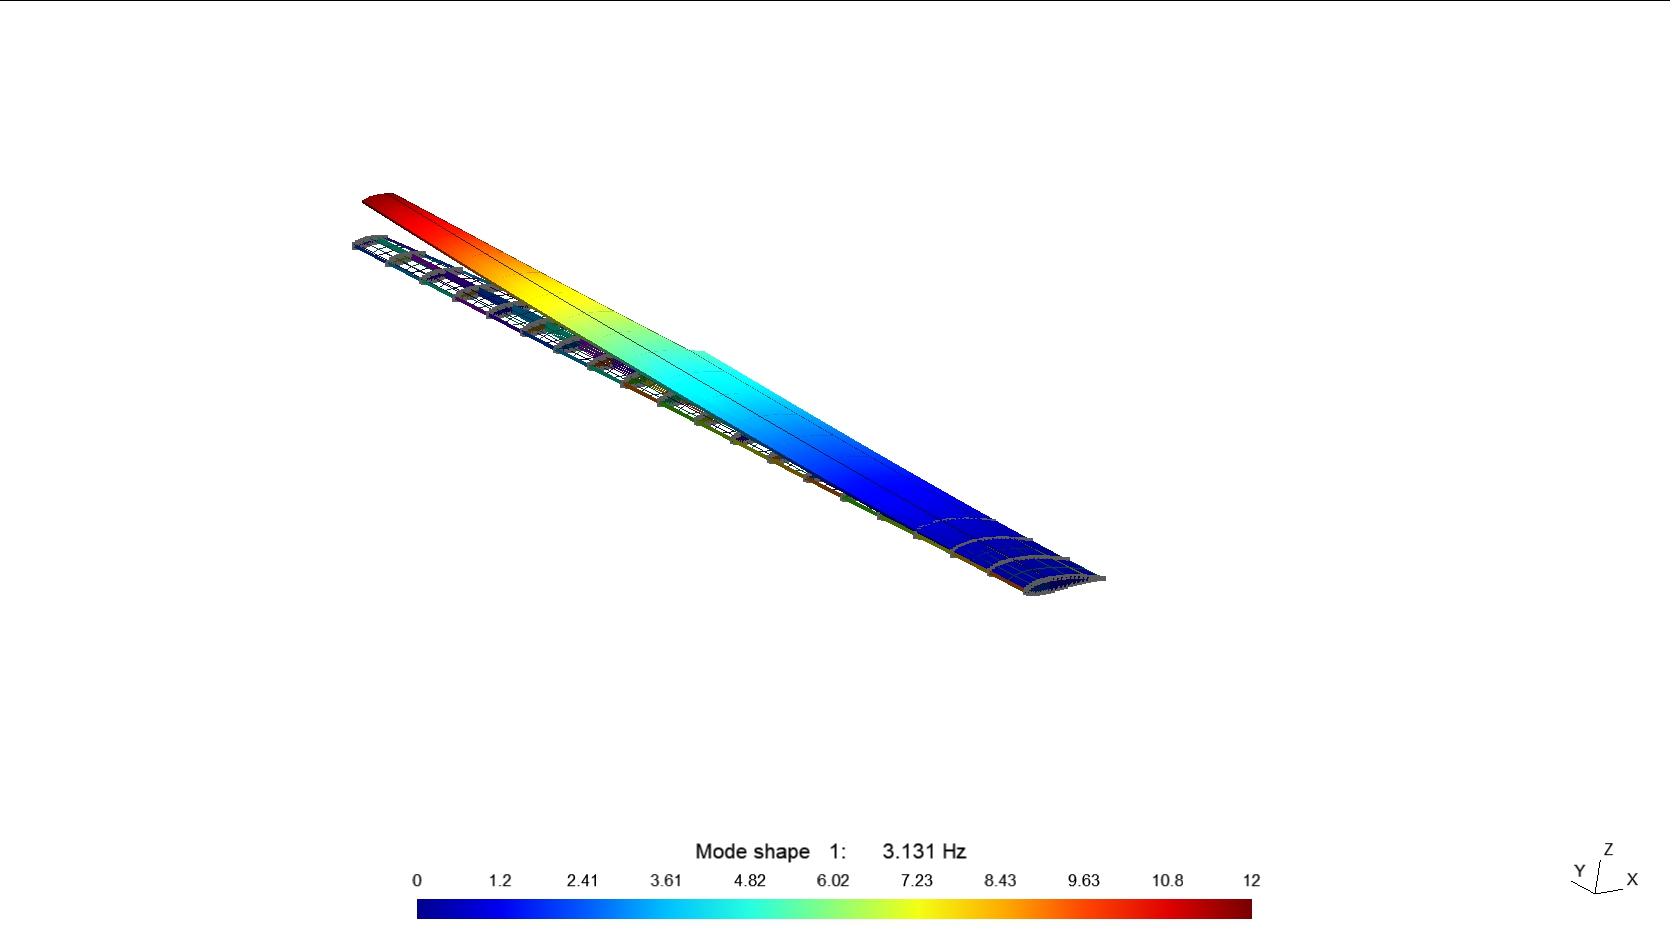
\includegraphics[width=\textwidth]{figures/mode1.jpg}
    \caption{The inverse relationship between probability and severity~\cite{CS-25}}
    \label{fig:inverseRelationship}
\end{figure}




